\Chapter{Project Implementation}

The GradeBadge application is designed to work on mobile, tablet devices and desktop computers. The UI of the application is developed using Bootstrap. When a page requires the data to be loaded from server or modified or deleted, a request is sent to the Web server over  HTTPS. The requests are sent to the Web server using Ajax. For handling Ajax requests and responses, this application uses JQuery Ajax API. All UI components are dynamically created or initialized in response to the data received from the Web server.

\newpage
\section{Loading Screen}
When the GradeBoard application is loaded, a loading screen is presented to the user as shown in the Figure ~\ref{fig:loading_screen}. The loading screen shows application logo and loading progess bar, and the screen is automatically redirected after the loading completed. 

\vspace{3em}
\begin{figure}[H]
\begin{center}
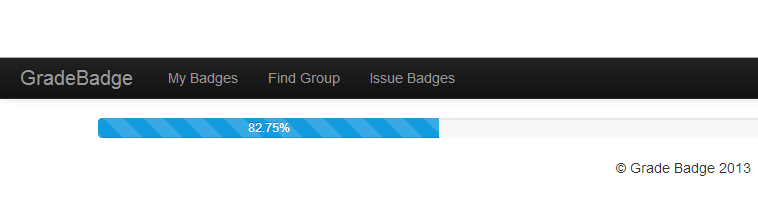
\includegraphics[height=3.8in,width=5.5in]{images/loading-screen.jpg}
\caption{GradeBadge Loading Screen}
\label{fig:loading_screen}
\end{center}
\end{figure}

\newpage
\section{Login Screen}
GradeBadge uses Facebook account for users to login. When the user is not logged-in to Facebook, the screen is automatically redirected to the Facebook login screen as shown in Figure~\ref{fig:login_screen}. Every user in the system can be badge issuer and badge earner.

\vspace{3em}
\begin{figure}[H]
\begin{center}
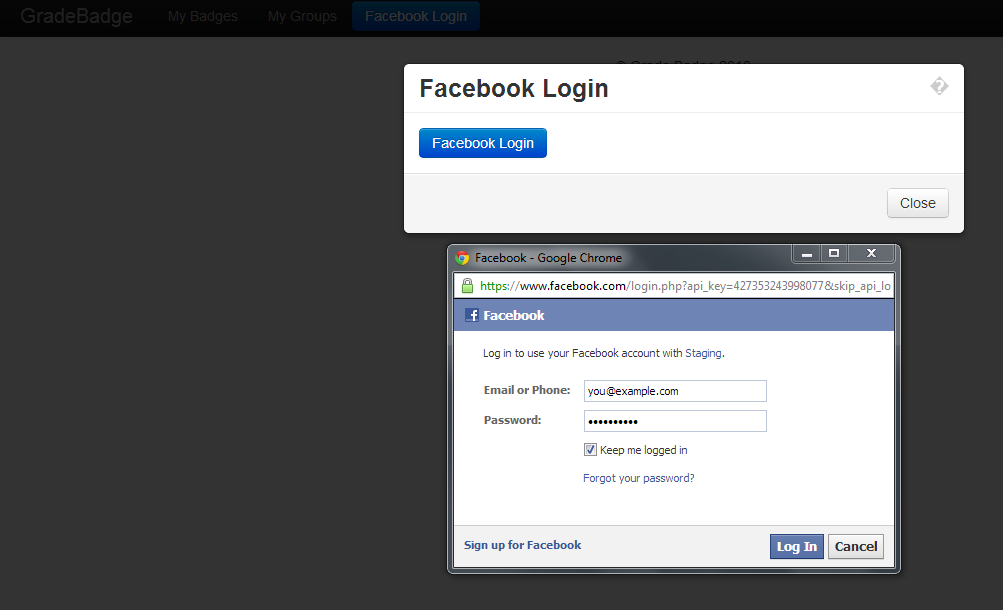
\includegraphics[height=3.3in,width=5.5in]{images/facebook-login.jpg}
\caption{GradeBadge Login Screen}
\label{fig:login_screen}
\end{center}
\end{figure}

\vspace{3em}
\begin{figure}[H]
\begin{center}
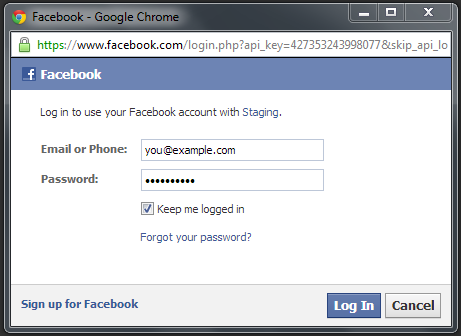
\includegraphics[height=3.8in,width=3.5in]{images/facebook-login1.jpg}
\caption{Facebook Login Screen}
\label{fig:fb_login_screen}
\end{center}
\end{figure}

\newpage
\section{Group Page}
 Badge issuers have access to list of groups that they manage as shown in Figure~\ref{fig:group-page1}. 

\vspace{3em}
\begin{figure}[H]
\begin{center}
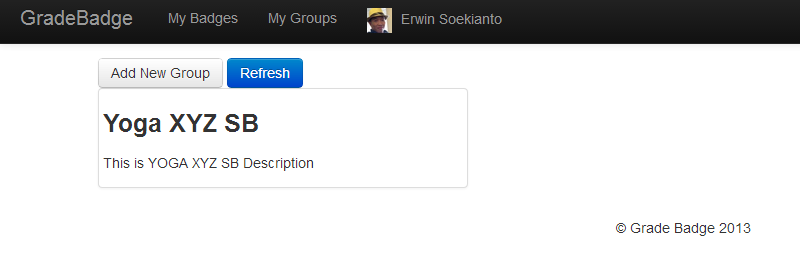
\includegraphics[height=3.1in,width=5.5in]{images/group-page1.png}
\caption{GradeBadge Group Page}
\label{fig:group-page1}
\end{center}
\end{figure}

\newpage
\section{Add New Group Page}
Badge issuers can add new group by clicking at "Add New Group" button in group page, then the pop-up modal window to create new group will appear  as shown in Figure~\ref{fig:add-new-group}. 

\vspace{3em}
\begin{figure}[H]
\begin{center}
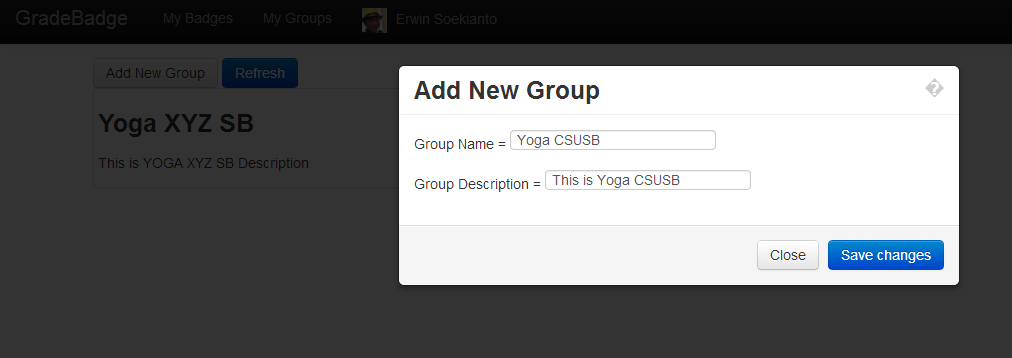
\includegraphics[height=3.1in,width=5.5in]{images/add-new-group.png}
\caption{GradeBadge Add New Group Page}
\label{fig:add-new-group}
\end{center}
\end{figure}

\newpage
\section{Group Page}
New groups have been added to group page as shown in Figure~\ref{fig:group-page2}. 

\vspace{3em}
\begin{figure}[H]
\begin{center}
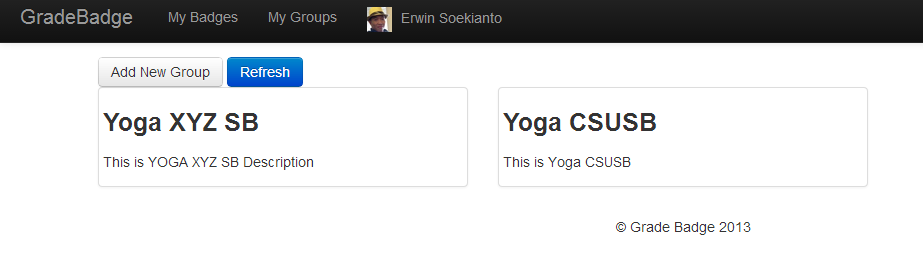
\includegraphics[height=6.1in,width=5.5in]{images/group-page2.png}
\caption{GradeBadge Group Page Added}
\label{fig:group-page2}
\end{center}
\end{figure}

\newpage
\section{Group Badge Page}
Badge issuers have access to list badges in a group by clicking at "Badge" button in a group thumbnail, then the application will display the list of badges in the selected group  as shown in Figure~\ref{fig:group-badge}. 

\vspace{3em}
\begin{figure}[H]
\begin{center}
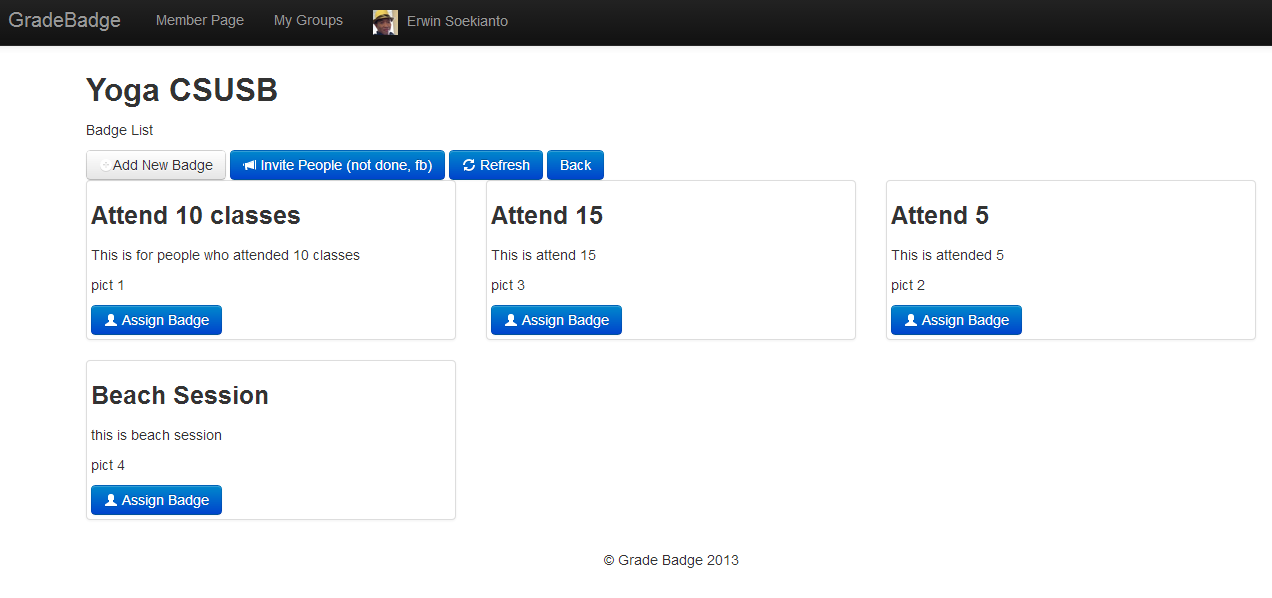
\includegraphics[height=5.1in,width=5.5in]{images/badge-page.png}
\caption{GradeBadge Group Badge Page}
\label{fig:group-badge}
\end{center}
\end{figure}

\newpage
\section{Add New Badge Page}
Badge issuers can add new badge by clicking at "Add New Badge" button in badge page, then the pop-up modal window to create new badge will appear  as shown in Figure~\ref{fig:add-new-badge}. 

\vspace{3em}
\begin{figure}[H]
\begin{center}
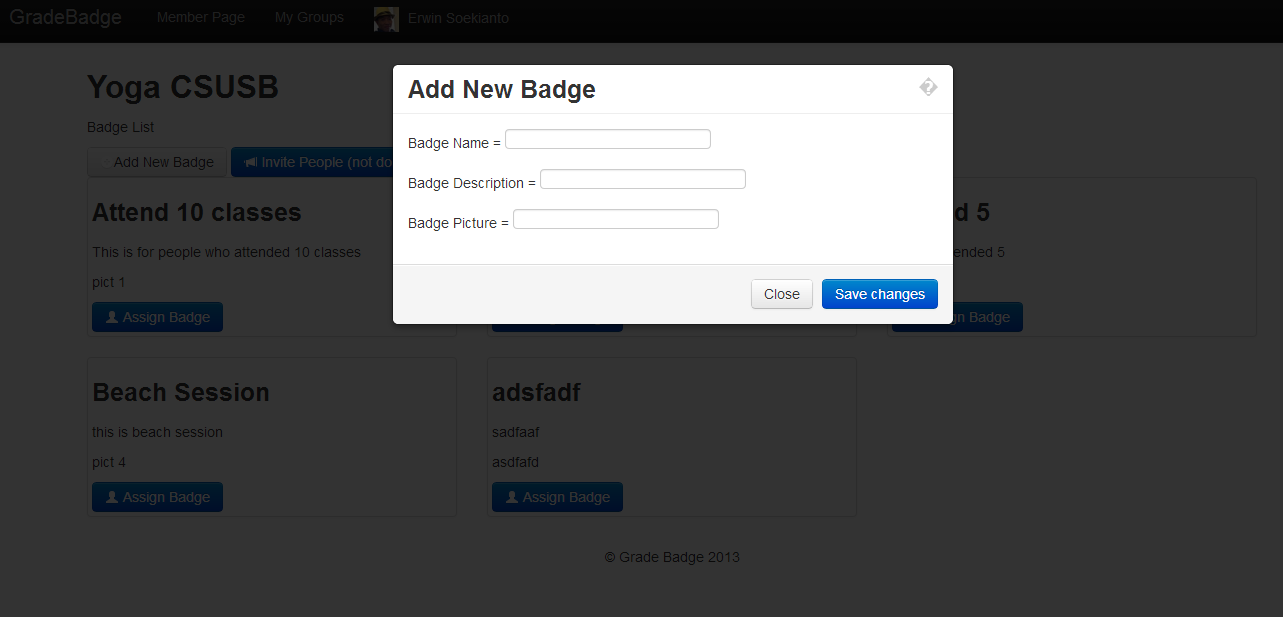
\includegraphics[height=5.1in,width=5.5in]{images/add-new-badge.png}
\caption{GradeBadge Add New Badge Page}
\label{fig:add-new-badge}
\end{center}
\end{figure}

\newpage
\section{Logging Counters Page}
The application also keeps track of errors, warnings and number of times a function is being callled. It can be accessed through web page as shown in Figure~\ref{fig:counters}. 

\vspace{3em}
\begin{figure}[H]
\begin{center}
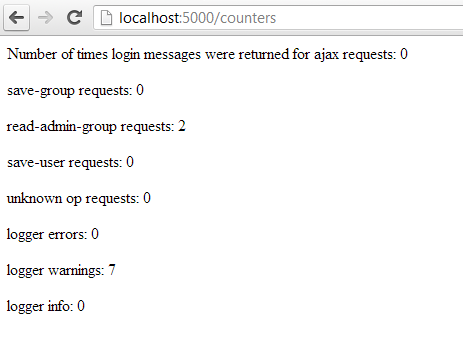
\includegraphics[height=3.1in,width=3.5in]{images/counters.png}
\caption{GradeBadge Logging Counters Page}
\label{fig:counters}
\end{center}
\end{figure}

\newpage
\section{Memory Statistic Page}
The application also monitors the memory and bandwidth usage of the application server. It can be accessed through web page as shown in Figure~\ref{fig:mem}. 

\vspace{3em}
\begin{figure}[H]
\begin{center}
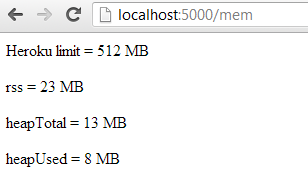
\includegraphics[height=3.1in,width=3.5in]{images/mem.png}
\caption{GradeBadge Memory Statistic Page}
\label{fig:mem}
\end{center}
\end{figure}



